% Created by tikzDevice version 0.12
% !TEX encoding = UTF-8 Unicode
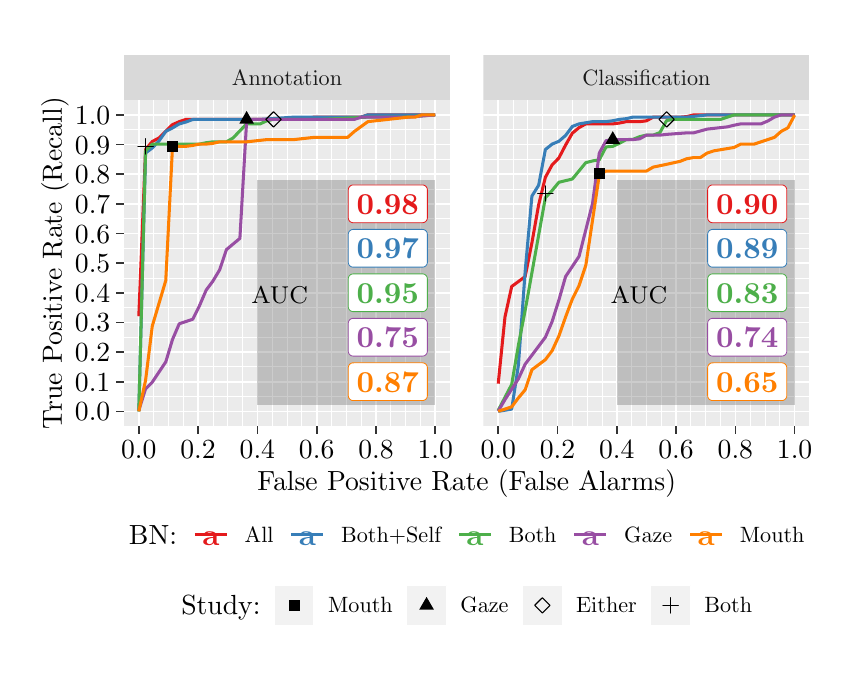
\begin{tikzpicture}[x=1pt,y=1pt]
\definecolor{fillColor}{RGB}{255,255,255}
\path[use as bounding box,fill=fillColor,fill opacity=0.00] (0,0) rectangle (288.00,231.38);
\begin{scope}
\path[clip] (  0.00,  4.41) rectangle (288.00,226.97);
\definecolor{drawColor}{RGB}{255,255,255}
\definecolor{fillColor}{RGB}{255,255,255}

\path[draw=drawColor,line width= 0.6pt,line join=round,line cap=round,fill=fillColor] (  0.00,  4.41) rectangle (288.00,226.97);
\end{scope}
\begin{scope}
\path[clip] ( 34.81, 87.39) rectangle (152.63,205.21);
\definecolor{fillColor}{gray}{0.92}

\path[fill=fillColor] ( 34.81, 87.39) rectangle (152.63,205.21);
\definecolor{drawColor}{RGB}{255,255,255}

\path[draw=drawColor,line width= 0.3pt,line join=round] ( 34.81, 98.10) --
	(152.63, 98.10);

\path[draw=drawColor,line width= 0.3pt,line join=round] ( 34.81,108.81) --
	(152.63,108.81);

\path[draw=drawColor,line width= 0.3pt,line join=round] ( 34.81,119.52) --
	(152.63,119.52);

\path[draw=drawColor,line width= 0.3pt,line join=round] ( 34.81,130.23) --
	(152.63,130.23);

\path[draw=drawColor,line width= 0.3pt,line join=round] ( 34.81,140.94) --
	(152.63,140.94);

\path[draw=drawColor,line width= 0.3pt,line join=round] ( 34.81,151.66) --
	(152.63,151.66);

\path[draw=drawColor,line width= 0.3pt,line join=round] ( 34.81,162.37) --
	(152.63,162.37);

\path[draw=drawColor,line width= 0.3pt,line join=round] ( 34.81,173.08) --
	(152.63,173.08);

\path[draw=drawColor,line width= 0.3pt,line join=round] ( 34.81,183.79) --
	(152.63,183.79);

\path[draw=drawColor,line width= 0.3pt,line join=round] ( 34.81,194.50) --
	(152.63,194.50);

\path[draw=drawColor,line width= 0.3pt,line join=round] ( 45.52, 87.39) --
	( 45.52,205.21);

\path[draw=drawColor,line width= 0.3pt,line join=round] ( 50.87, 87.39) --
	( 50.87,205.21);

\path[draw=drawColor,line width= 0.3pt,line join=round] ( 56.23, 87.39) --
	( 56.23,205.21);

\path[draw=drawColor,line width= 0.3pt,line join=round] ( 66.94, 87.39) --
	( 66.94,205.21);

\path[draw=drawColor,line width= 0.3pt,line join=round] ( 72.30, 87.39) --
	( 72.30,205.21);

\path[draw=drawColor,line width= 0.3pt,line join=round] ( 77.65, 87.39) --
	( 77.65,205.21);

\path[draw=drawColor,line width= 0.3pt,line join=round] ( 88.36, 87.39) --
	( 88.36,205.21);

\path[draw=drawColor,line width= 0.3pt,line join=round] ( 93.72, 87.39) --
	( 93.72,205.21);

\path[draw=drawColor,line width= 0.3pt,line join=round] ( 99.07, 87.39) --
	( 99.07,205.21);

\path[draw=drawColor,line width= 0.3pt,line join=round] (109.79, 87.39) --
	(109.79,205.21);

\path[draw=drawColor,line width= 0.3pt,line join=round] (115.14, 87.39) --
	(115.14,205.21);

\path[draw=drawColor,line width= 0.3pt,line join=round] (120.50, 87.39) --
	(120.50,205.21);

\path[draw=drawColor,line width= 0.3pt,line join=round] (131.21, 87.39) --
	(131.21,205.21);

\path[draw=drawColor,line width= 0.3pt,line join=round] (136.56, 87.39) --
	(136.56,205.21);

\path[draw=drawColor,line width= 0.3pt,line join=round] (141.92, 87.39) --
	(141.92,205.21);

\path[draw=drawColor,line width= 0.6pt,line join=round] ( 34.81, 92.74) --
	(152.63, 92.74);

\path[draw=drawColor,line width= 0.6pt,line join=round] ( 34.81,103.45) --
	(152.63,103.45);

\path[draw=drawColor,line width= 0.6pt,line join=round] ( 34.81,114.17) --
	(152.63,114.17);

\path[draw=drawColor,line width= 0.6pt,line join=round] ( 34.81,124.88) --
	(152.63,124.88);

\path[draw=drawColor,line width= 0.6pt,line join=round] ( 34.81,135.59) --
	(152.63,135.59);

\path[draw=drawColor,line width= 0.6pt,line join=round] ( 34.81,146.30) --
	(152.63,146.30);

\path[draw=drawColor,line width= 0.6pt,line join=round] ( 34.81,157.01) --
	(152.63,157.01);

\path[draw=drawColor,line width= 0.6pt,line join=round] ( 34.81,167.72) --
	(152.63,167.72);

\path[draw=drawColor,line width= 0.6pt,line join=round] ( 34.81,178.43) --
	(152.63,178.43);

\path[draw=drawColor,line width= 0.6pt,line join=round] ( 34.81,189.15) --
	(152.63,189.15);

\path[draw=drawColor,line width= 0.6pt,line join=round] ( 34.81,199.86) --
	(152.63,199.86);

\path[draw=drawColor,line width= 0.6pt,line join=round] ( 40.16, 87.39) --
	( 40.16,205.21);

\path[draw=drawColor,line width= 0.6pt,line join=round] ( 61.58, 87.39) --
	( 61.58,205.21);

\path[draw=drawColor,line width= 0.6pt,line join=round] ( 83.01, 87.39) --
	( 83.01,205.21);

\path[draw=drawColor,line width= 0.6pt,line join=round] (104.43, 87.39) --
	(104.43,205.21);

\path[draw=drawColor,line width= 0.6pt,line join=round] (125.85, 87.39) --
	(125.85,205.21);

\path[draw=drawColor,line width= 0.6pt,line join=round] (147.27, 87.39) --
	(147.27,205.21);
\definecolor{fillColor}{RGB}{89,89,89}

\path[fill=fillColor,fill opacity=0.30] ( 83.01, 94.89) rectangle (147.27,176.29);
\definecolor{drawColor}{RGB}{0,0,0}

\node[text=drawColor,anchor=base,inner sep=0pt, outer sep=0pt, scale=  1.10] at ( 91.04,131.79) {\footnotesize{AUC}};
\definecolor{drawColor}{RGB}{255,127,0}
\definecolor{fillColor}{RGB}{255,255,255}

\path[draw=drawColor,line width= 0.3pt,line join=round,line cap=round,fill=fillColor] (117.65, 96.63) --
	(142.62, 96.63) --
	(142.55, 96.64) --
	(142.84, 96.65) --
	(143.13, 96.71) --
	(143.40, 96.81) --
	(143.65, 96.95) --
	(143.88, 97.14) --
	(144.07, 97.36) --
	(144.22, 97.60) --
	(144.34, 97.87) --
	(144.41, 98.15) --
	(144.43, 98.44) --
	(144.43, 98.44) --
	(144.43,108.47) --
	(144.43,108.47) --
	(144.41,108.76) --
	(144.34,109.04) --
	(144.22,109.31) --
	(144.07,109.55) --
	(143.88,109.77) --
	(143.65,109.96) --
	(143.40,110.10) --
	(143.13,110.20) --
	(142.84,110.26) --
	(142.62,110.28) --
	(117.65,110.28) --
	(117.87,110.26) --
	(117.58,110.27) --
	(117.29,110.24) --
	(117.01,110.16) --
	(116.75,110.03) --
	(116.51,109.87) --
	(116.30,109.67) --
	(116.12,109.43) --
	(115.99,109.18) --
	(115.90,108.90) --
	(115.85,108.61) --
	(115.84,108.47) --
	(115.84, 98.44) --
	(115.85, 98.59) --
	(115.85, 98.30) --
	(115.90, 98.01) --
	(115.99, 97.73) --
	(116.12, 97.48) --
	(116.30, 97.24) --
	(116.51, 97.04) --
	(116.75, 96.88) --
	(117.01, 96.75) --
	(117.29, 96.67) --
	(117.58, 96.64) --
	cycle;
\end{scope}
\begin{scope}
\path[clip] ( 34.81, 87.39) rectangle (152.63,205.21);
\definecolor{drawColor}{RGB}{255,127,0}

\node[text=drawColor,anchor=base,inner sep=0pt, outer sep=0pt, scale=  1.10] at (130.14, 99.65) {\bfseries 0.87};
\definecolor{drawColor}{RGB}{152,78,163}
\definecolor{fillColor}{RGB}{255,255,255}

\path[draw=drawColor,line width= 0.3pt,line join=round,line cap=round,fill=fillColor] (117.65,112.70) --
	(142.62,112.70) --
	(142.55,112.70) --
	(142.84,112.71) --
	(143.13,112.77) --
	(143.40,112.88) --
	(143.65,113.02) --
	(143.88,113.20) --
	(144.07,113.42) --
	(144.22,113.67) --
	(144.34,113.94) --
	(144.41,114.22) --
	(144.43,114.51) --
	(144.43,114.51) --
	(144.43,124.54) --
	(144.43,124.54) --
	(144.41,124.83) --
	(144.34,125.11) --
	(144.22,125.38) --
	(144.07,125.62) --
	(143.88,125.84) --
	(143.65,126.02) --
	(143.40,126.17) --
	(143.13,126.27) --
	(142.84,126.33) --
	(142.62,126.34) --
	(117.65,126.34) --
	(117.87,126.33) --
	(117.58,126.34) --
	(117.29,126.31) --
	(117.01,126.23) --
	(116.75,126.10) --
	(116.51,125.94) --
	(116.30,125.73) --
	(116.12,125.50) --
	(115.99,125.24) --
	(115.90,124.97) --
	(115.85,124.68) --
	(115.84,124.54) --
	(115.84,114.51) --
	(115.85,114.65) --
	(115.85,114.36) --
	(115.90,114.08) --
	(115.99,113.80) --
	(116.12,113.54) --
	(116.30,113.31) --
	(116.51,113.11) --
	(116.75,112.94) --
	(117.01,112.82) --
	(117.29,112.74) --
	(117.58,112.70) --
	cycle;
\end{scope}
\begin{scope}
\path[clip] ( 34.81, 87.39) rectangle (152.63,205.21);
\definecolor{drawColor}{RGB}{152,78,163}

\node[text=drawColor,anchor=base,inner sep=0pt, outer sep=0pt, scale=  1.10] at (130.14,115.71) {\bfseries 0.75};
\definecolor{drawColor}{RGB}{77,175,74}
\definecolor{fillColor}{RGB}{255,255,255}

\path[draw=drawColor,line width= 0.3pt,line join=round,line cap=round,fill=fillColor] (117.65,128.77) --
	(142.62,128.77) --
	(142.55,128.77) --
	(142.84,128.78) --
	(143.13,128.84) --
	(143.40,128.94) --
	(143.65,129.09) --
	(143.88,129.27) --
	(144.07,129.49) --
	(144.22,129.74) --
	(144.34,130.00) --
	(144.41,130.29) --
	(144.43,130.57) --
	(144.43,130.57) --
	(144.43,140.60) --
	(144.43,140.60) --
	(144.41,140.89) --
	(144.34,141.17) --
	(144.22,141.44) --
	(144.07,141.69) --
	(143.88,141.91) --
	(143.65,142.09) --
	(143.40,142.24) --
	(143.13,142.34) --
	(142.84,142.40) --
	(142.62,142.41) --
	(117.65,142.41) --
	(117.87,142.40) --
	(117.58,142.41) --
	(117.29,142.37) --
	(117.01,142.29) --
	(116.75,142.17) --
	(116.51,142.00) --
	(116.30,141.80) --
	(116.12,141.57) --
	(115.99,141.31) --
	(115.90,141.04) --
	(115.85,140.75) --
	(115.84,140.60) --
	(115.84,130.57) --
	(115.85,130.72) --
	(115.85,130.43) --
	(115.90,130.14) --
	(115.99,129.87) --
	(116.12,129.61) --
	(116.30,129.38) --
	(116.51,129.18) --
	(116.75,129.01) --
	(117.01,128.89) --
	(117.29,128.80) --
	(117.58,128.77) --
	cycle;
\end{scope}
\begin{scope}
\path[clip] ( 34.81, 87.39) rectangle (152.63,205.21);
\definecolor{drawColor}{RGB}{77,175,74}

\node[text=drawColor,anchor=base,inner sep=0pt, outer sep=0pt, scale=  1.10] at (130.14,131.78) {\bfseries 0.95};
\definecolor{drawColor}{RGB}{55,126,184}
\definecolor{fillColor}{RGB}{255,255,255}

\path[draw=drawColor,line width= 0.3pt,line join=round,line cap=round,fill=fillColor] (117.65,144.84) --
	(142.62,144.84) --
	(142.55,144.84) --
	(142.84,144.85) --
	(143.13,144.91) --
	(143.40,145.01) --
	(143.65,145.15) --
	(143.88,145.34) --
	(144.07,145.56) --
	(144.22,145.80) --
	(144.34,146.07) --
	(144.41,146.35) --
	(144.43,146.64) --
	(144.43,146.64) --
	(144.43,156.67) --
	(144.43,156.67) --
	(144.41,156.96) --
	(144.34,157.24) --
	(144.22,157.51) --
	(144.07,157.76) --
	(143.88,157.97) --
	(143.65,158.16) --
	(143.40,158.30) --
	(143.13,158.41) --
	(142.84,158.46) --
	(142.62,158.48) --
	(117.65,158.48) --
	(117.87,158.46) --
	(117.58,158.48) --
	(117.29,158.44) --
	(117.01,158.36) --
	(116.75,158.23) --
	(116.51,158.07) --
	(116.30,157.87) --
	(116.12,157.64) --
	(115.99,157.38) --
	(115.90,157.10) --
	(115.85,156.82) --
	(115.84,156.67) --
	(115.84,146.64) --
	(115.85,146.79) --
	(115.85,146.50) --
	(115.90,146.21) --
	(115.99,145.93) --
	(116.12,145.68) --
	(116.30,145.44) --
	(116.51,145.24) --
	(116.75,145.08) --
	(117.01,144.95) --
	(117.29,144.87) --
	(117.58,144.84) --
	cycle;
\end{scope}
\begin{scope}
\path[clip] ( 34.81, 87.39) rectangle (152.63,205.21);
\definecolor{drawColor}{RGB}{55,126,184}

\node[text=drawColor,anchor=base,inner sep=0pt, outer sep=0pt, scale=  1.10] at (130.14,147.85) {\bfseries 0.97};
\definecolor{drawColor}{RGB}{228,26,28}
\definecolor{fillColor}{RGB}{255,255,255}

\path[draw=drawColor,line width= 0.3pt,line join=round,line cap=round,fill=fillColor] (117.65,160.90) --
	(142.62,160.90) --
	(142.55,160.90) --
	(142.84,160.92) --
	(143.13,160.97) --
	(143.40,161.08) --
	(143.65,161.22) --
	(143.88,161.41) --
	(144.07,161.62) --
	(144.22,161.87) --
	(144.34,162.14) --
	(144.41,162.42) --
	(144.43,162.71) --
	(144.43,162.71) --
	(144.43,172.74) --
	(144.43,172.74) --
	(144.41,173.03) --
	(144.34,173.31) --
	(144.22,173.58) --
	(144.07,173.82) --
	(143.88,174.04) --
	(143.65,174.22) --
	(143.40,174.37) --
	(143.13,174.47) --
	(142.84,174.53) --
	(142.62,174.54) --
	(117.65,174.54) --
	(117.87,174.53) --
	(117.58,174.54) --
	(117.29,174.51) --
	(117.01,174.43) --
	(116.75,174.30) --
	(116.51,174.14) --
	(116.30,173.93) --
	(116.12,173.70) --
	(115.99,173.44) --
	(115.90,173.17) --
	(115.85,172.88) --
	(115.84,172.74) --
	(115.84,162.71) --
	(115.85,162.85) --
	(115.85,162.56) --
	(115.90,162.28) --
	(115.99,162.00) --
	(116.12,161.74) --
	(116.30,161.51) --
	(116.51,161.31) --
	(116.75,161.14) --
	(117.01,161.02) --
	(117.29,160.94) --
	(117.58,160.90) --
	cycle;
\end{scope}
\begin{scope}
\path[clip] ( 34.81, 87.39) rectangle (152.63,205.21);
\definecolor{drawColor}{RGB}{228,26,28}

\node[text=drawColor,anchor=base,inner sep=0pt, outer sep=0pt, scale=  1.10] at (130.14,163.91) {\bfseries 0.98};

\path[draw=drawColor,line width= 1.1pt,line join=round] ( 40.16,127.10) --
	( 42.60,187.38) --
	( 45.03,190.25) --
	( 47.46,191.54) --
	( 49.90,193.91) --
	( 52.33,196.34) --
	( 54.77,197.42) --
	( 57.20,198.23) --
	( 59.64,198.23) --
	( 62.07,198.23) --
	( 64.51,198.23) --
	( 66.94,198.23) --
	( 74.24,198.23) --
	( 76.68,198.23) --
	( 79.11,198.23) --
	( 81.55,198.23) --
	( 83.98,198.23) --
	( 91.28,198.23) --
	( 93.72,198.23) --
	( 98.59,198.23) --
	(103.46,199.05) --
	(110.76,199.05) --
	(120.50,199.05) --
	(122.93,199.86) --
	(125.37,199.86) --
	(147.27,199.86);
\definecolor{drawColor}{RGB}{55,126,184}

\path[draw=drawColor,line width= 1.1pt,line join=round] ( 40.16, 92.74) --
	( 42.60,186.07) --
	( 45.03,187.92) --
	( 47.46,190.47) --
	( 49.90,193.89) --
	( 52.33,195.14) --
	( 54.77,196.61) --
	( 57.20,197.28) --
	( 59.64,198.20) --
	( 62.07,198.23) --
	( 64.51,198.23) --
	( 69.37,198.23) --
	( 71.81,198.23) --
	( 74.24,198.23) --
	( 83.98,198.23) --
	( 96.15,199.05) --
	(108.32,199.05) --
	(110.76,199.05) --
	(113.19,199.05) --
	(118.06,199.05) --
	(120.50,199.05) --
	(122.93,199.86) --
	(147.27,199.86);
\definecolor{drawColor}{RGB}{77,175,74}

\path[draw=drawColor,line width= 1.1pt,line join=round] ( 40.16, 92.74) --
	( 42.60,186.80) --
	( 45.03,189.31) --
	( 47.46,189.31) --
	( 49.90,189.31) --
	( 57.20,189.31) --
	( 59.64,189.31) --
	( 62.07,189.31) --
	( 64.51,189.81) --
	( 66.94,190.12) --
	( 69.37,190.12) --
	( 71.81,190.12) --
	( 74.24,191.54) --
	( 76.68,194.10) --
	( 79.11,196.61) --
	( 81.55,196.61) --
	( 83.98,196.61) --
	( 86.41,197.72) --
	( 88.85,198.23) --
	( 96.15,198.23) --
	(105.89,198.23) --
	(122.93,199.05) --
	(135.10,199.05) --
	(147.27,199.86);
\definecolor{drawColor}{RGB}{152,78,163}

\path[draw=drawColor,line width= 1.1pt,line join=round] ( 40.16, 93.08) --
	( 42.60,100.86) --
	( 45.03,103.29) --
	( 49.90,110.60) --
	( 52.33,118.71) --
	( 54.77,124.39) --
	( 59.64,126.01) --
	( 62.07,130.88) --
	( 64.51,136.56) --
	( 66.94,139.81) --
	( 69.37,143.87) --
	( 71.81,151.17) --
	( 76.68,155.23) --
	( 79.11,197.51) --
	( 81.55,198.23) --
	( 83.98,198.23) --
	( 88.85,198.23) --
	( 91.28,198.23) --
	( 96.15,198.23) --
	(101.02,198.23) --
	(105.89,198.23) --
	(108.32,198.23) --
	(110.76,198.23) --
	(115.63,198.23) --
	(118.06,198.23) --
	(120.50,199.05) --
	(122.93,199.05) --
	(127.80,199.05) --
	(132.67,199.05) --
	(137.54,199.05) --
	(142.41,199.45) --
	(147.27,199.86);
\definecolor{drawColor}{RGB}{255,127,0}

\path[draw=drawColor,line width= 1.1pt,line join=round] ( 40.16, 92.74) --
	( 42.60,103.94) --
	( 45.03,123.58) --
	( 49.90,140.01) --
	( 52.33,188.31) --
	( 54.77,188.50) --
	( 57.20,188.50) --
	( 59.64,188.82) --
	( 62.07,189.31) --
	( 64.51,189.31) --
	( 66.94,189.58) --
	( 69.37,190.12) --
	( 71.81,190.12) --
	( 74.24,190.12) --
	( 79.11,190.12) --
	( 86.41,190.93) --
	( 88.85,190.93) --
	( 91.28,190.93) --
	( 93.72,190.93) --
	( 96.15,190.93) --
	(103.46,191.74) --
	(105.89,191.74) --
	(108.32,191.74) --
	(110.76,191.74) --
	(113.19,191.74) --
	(115.63,191.74) --
	(118.06,193.89) --
	(122.93,197.42) --
	(130.23,198.23) --
	(137.54,199.05) --
	(139.97,199.05) --
	(142.41,199.86) --
	(144.84,199.86) --
	(147.27,199.86);
\definecolor{fillColor}{RGB}{0,0,0}

\path[fill=fillColor] ( 79.11,201.29) --
	( 81.75,196.71) --
	( 76.47,196.71) --
	cycle;

\path[fill=fillColor] ( 50.37,186.53) --
	( 54.30,186.53) --
	( 54.30,190.46) --
	( 50.37,190.46) --
	cycle;
\definecolor{drawColor}{RGB}{0,0,0}

\path[draw=drawColor,line width= 0.4pt,line join=round,line cap=round] ( 39.82,188.50) -- ( 45.37,188.50);

\path[draw=drawColor,line width= 0.4pt,line join=round,line cap=round] ( 42.60,185.72) -- ( 42.60,191.27);

\path[draw=drawColor,line width= 0.4pt,line join=round,line cap=round] ( 86.07,198.23) --
	( 88.85,201.01) --
	( 91.62,198.23) --
	( 88.85,195.46) --
	( 86.07,198.23);
\end{scope}
\begin{scope}
\path[clip] (164.68, 87.39) rectangle (282.50,205.21);
\definecolor{fillColor}{gray}{0.92}

\path[fill=fillColor] (164.68, 87.39) rectangle (282.50,205.21);
\definecolor{drawColor}{RGB}{255,255,255}

\path[draw=drawColor,line width= 0.3pt,line join=round] (164.68, 98.10) --
	(282.50, 98.10);

\path[draw=drawColor,line width= 0.3pt,line join=round] (164.68,108.81) --
	(282.50,108.81);

\path[draw=drawColor,line width= 0.3pt,line join=round] (164.68,119.52) --
	(282.50,119.52);

\path[draw=drawColor,line width= 0.3pt,line join=round] (164.68,130.23) --
	(282.50,130.23);

\path[draw=drawColor,line width= 0.3pt,line join=round] (164.68,140.94) --
	(282.50,140.94);

\path[draw=drawColor,line width= 0.3pt,line join=round] (164.68,151.66) --
	(282.50,151.66);

\path[draw=drawColor,line width= 0.3pt,line join=round] (164.68,162.37) --
	(282.50,162.37);

\path[draw=drawColor,line width= 0.3pt,line join=round] (164.68,173.08) --
	(282.50,173.08);

\path[draw=drawColor,line width= 0.3pt,line join=round] (164.68,183.79) --
	(282.50,183.79);

\path[draw=drawColor,line width= 0.3pt,line join=round] (164.68,194.50) --
	(282.50,194.50);

\path[draw=drawColor,line width= 0.3pt,line join=round] (175.39, 87.39) --
	(175.39,205.21);

\path[draw=drawColor,line width= 0.3pt,line join=round] (180.74, 87.39) --
	(180.74,205.21);

\path[draw=drawColor,line width= 0.3pt,line join=round] (186.10, 87.39) --
	(186.10,205.21);

\path[draw=drawColor,line width= 0.3pt,line join=round] (196.81, 87.39) --
	(196.81,205.21);

\path[draw=drawColor,line width= 0.3pt,line join=round] (202.17, 87.39) --
	(202.17,205.21);

\path[draw=drawColor,line width= 0.3pt,line join=round] (207.52, 87.39) --
	(207.52,205.21);

\path[draw=drawColor,line width= 0.3pt,line join=round] (218.23, 87.39) --
	(218.23,205.21);

\path[draw=drawColor,line width= 0.3pt,line join=round] (223.59, 87.39) --
	(223.59,205.21);

\path[draw=drawColor,line width= 0.3pt,line join=round] (228.94, 87.39) --
	(228.94,205.21);

\path[draw=drawColor,line width= 0.3pt,line join=round] (239.65, 87.39) --
	(239.65,205.21);

\path[draw=drawColor,line width= 0.3pt,line join=round] (245.01, 87.39) --
	(245.01,205.21);

\path[draw=drawColor,line width= 0.3pt,line join=round] (250.37, 87.39) --
	(250.37,205.21);

\path[draw=drawColor,line width= 0.3pt,line join=round] (261.08, 87.39) --
	(261.08,205.21);

\path[draw=drawColor,line width= 0.3pt,line join=round] (266.43, 87.39) --
	(266.43,205.21);

\path[draw=drawColor,line width= 0.3pt,line join=round] (271.79, 87.39) --
	(271.79,205.21);

\path[draw=drawColor,line width= 0.6pt,line join=round] (164.68, 92.74) --
	(282.50, 92.74);

\path[draw=drawColor,line width= 0.6pt,line join=round] (164.68,103.45) --
	(282.50,103.45);

\path[draw=drawColor,line width= 0.6pt,line join=round] (164.68,114.17) --
	(282.50,114.17);

\path[draw=drawColor,line width= 0.6pt,line join=round] (164.68,124.88) --
	(282.50,124.88);

\path[draw=drawColor,line width= 0.6pt,line join=round] (164.68,135.59) --
	(282.50,135.59);

\path[draw=drawColor,line width= 0.6pt,line join=round] (164.68,146.30) --
	(282.50,146.30);

\path[draw=drawColor,line width= 0.6pt,line join=round] (164.68,157.01) --
	(282.50,157.01);

\path[draw=drawColor,line width= 0.6pt,line join=round] (164.68,167.72) --
	(282.50,167.72);

\path[draw=drawColor,line width= 0.6pt,line join=round] (164.68,178.43) --
	(282.50,178.43);

\path[draw=drawColor,line width= 0.6pt,line join=round] (164.68,189.15) --
	(282.50,189.15);

\path[draw=drawColor,line width= 0.6pt,line join=round] (164.68,199.86) --
	(282.50,199.86);

\path[draw=drawColor,line width= 0.6pt,line join=round] (170.03, 87.39) --
	(170.03,205.21);

\path[draw=drawColor,line width= 0.6pt,line join=round] (191.45, 87.39) --
	(191.45,205.21);

\path[draw=drawColor,line width= 0.6pt,line join=round] (212.88, 87.39) --
	(212.88,205.21);

\path[draw=drawColor,line width= 0.6pt,line join=round] (234.30, 87.39) --
	(234.30,205.21);

\path[draw=drawColor,line width= 0.6pt,line join=round] (255.72, 87.39) --
	(255.72,205.21);

\path[draw=drawColor,line width= 0.6pt,line join=round] (277.14, 87.39) --
	(277.14,205.21);
\definecolor{fillColor}{RGB}{89,89,89}

\path[fill=fillColor,fill opacity=0.30] (212.88, 94.89) rectangle (277.14,176.29);
\definecolor{drawColor}{RGB}{0,0,0}

\node[text=drawColor,anchor=base,inner sep=0pt, outer sep=0pt, scale=  1.10] at (220.91,131.79) {\footnotesize{AUC}};
\definecolor{drawColor}{RGB}{255,127,0}
\definecolor{fillColor}{RGB}{255,255,255}

\path[draw=drawColor,line width= 0.3pt,line join=round,line cap=round,fill=fillColor] (247.52, 96.63) --
	(272.49, 96.63) --
	(272.42, 96.64) --
	(272.71, 96.65) --
	(273.00, 96.71) --
	(273.27, 96.81) --
	(273.52, 96.95) --
	(273.74, 97.14) --
	(273.94, 97.36) --
	(274.09, 97.60) --
	(274.21, 97.87) --
	(274.28, 98.15) --
	(274.30, 98.44) --
	(274.30, 98.44) --
	(274.30,108.47) --
	(274.30,108.47) --
	(274.28,108.76) --
	(274.21,109.04) --
	(274.09,109.31) --
	(273.94,109.55) --
	(273.74,109.77) --
	(273.52,109.96) --
	(273.27,110.10) --
	(273.00,110.20) --
	(272.71,110.26) --
	(272.49,110.28) --
	(247.52,110.28) --
	(247.74,110.26) --
	(247.45,110.27) --
	(247.16,110.24) --
	(246.88,110.16) --
	(246.62,110.03) --
	(246.38,109.87) --
	(246.17,109.67) --
	(245.99,109.43) --
	(245.86,109.18) --
	(245.76,108.90) --
	(245.72,108.61) --
	(245.71,108.47) --
	(245.71, 98.44) --
	(245.72, 98.59) --
	(245.72, 98.30) --
	(245.76, 98.01) --
	(245.86, 97.73) --
	(245.99, 97.48) --
	(246.17, 97.24) --
	(246.38, 97.04) --
	(246.62, 96.88) --
	(246.88, 96.75) --
	(247.16, 96.67) --
	(247.45, 96.64) --
	cycle;
\end{scope}
\begin{scope}
\path[clip] (164.68, 87.39) rectangle (282.50,205.21);
\definecolor{drawColor}{RGB}{255,127,0}

\node[text=drawColor,anchor=base,inner sep=0pt, outer sep=0pt, scale=  1.10] at (260.01, 99.65) {\bfseries 0.65};
\definecolor{drawColor}{RGB}{152,78,163}
\definecolor{fillColor}{RGB}{255,255,255}

\path[draw=drawColor,line width= 0.3pt,line join=round,line cap=round,fill=fillColor] (247.52,112.70) --
	(272.49,112.70) --
	(272.42,112.70) --
	(272.71,112.71) --
	(273.00,112.77) --
	(273.27,112.88) --
	(273.52,113.02) --
	(273.74,113.20) --
	(273.94,113.42) --
	(274.09,113.67) --
	(274.21,113.94) --
	(274.28,114.22) --
	(274.30,114.51) --
	(274.30,114.51) --
	(274.30,124.54) --
	(274.30,124.54) --
	(274.28,124.83) --
	(274.21,125.11) --
	(274.09,125.38) --
	(273.94,125.62) --
	(273.74,125.84) --
	(273.52,126.02) --
	(273.27,126.17) --
	(273.00,126.27) --
	(272.71,126.33) --
	(272.49,126.34) --
	(247.52,126.34) --
	(247.74,126.33) --
	(247.45,126.34) --
	(247.16,126.31) --
	(246.88,126.23) --
	(246.62,126.10) --
	(246.38,125.94) --
	(246.17,125.73) --
	(245.99,125.50) --
	(245.86,125.24) --
	(245.76,124.97) --
	(245.72,124.68) --
	(245.71,124.54) --
	(245.71,114.51) --
	(245.72,114.65) --
	(245.72,114.36) --
	(245.76,114.08) --
	(245.86,113.80) --
	(245.99,113.54) --
	(246.17,113.31) --
	(246.38,113.11) --
	(246.62,112.94) --
	(246.88,112.82) --
	(247.16,112.74) --
	(247.45,112.70) --
	cycle;
\end{scope}
\begin{scope}
\path[clip] (164.68, 87.39) rectangle (282.50,205.21);
\definecolor{drawColor}{RGB}{152,78,163}

\node[text=drawColor,anchor=base,inner sep=0pt, outer sep=0pt, scale=  1.10] at (260.01,115.71) {\bfseries 0.74};
\definecolor{drawColor}{RGB}{77,175,74}
\definecolor{fillColor}{RGB}{255,255,255}

\path[draw=drawColor,line width= 0.3pt,line join=round,line cap=round,fill=fillColor] (247.52,128.77) --
	(272.49,128.77) --
	(272.42,128.77) --
	(272.71,128.78) --
	(273.00,128.84) --
	(273.27,128.94) --
	(273.52,129.09) --
	(273.74,129.27) --
	(273.94,129.49) --
	(274.09,129.74) --
	(274.21,130.00) --
	(274.28,130.29) --
	(274.30,130.57) --
	(274.30,130.57) --
	(274.30,140.60) --
	(274.30,140.60) --
	(274.28,140.89) --
	(274.21,141.17) --
	(274.09,141.44) --
	(273.94,141.69) --
	(273.74,141.91) --
	(273.52,142.09) --
	(273.27,142.24) --
	(273.00,142.34) --
	(272.71,142.40) --
	(272.49,142.41) --
	(247.52,142.41) --
	(247.74,142.40) --
	(247.45,142.41) --
	(247.16,142.37) --
	(246.88,142.29) --
	(246.62,142.17) --
	(246.38,142.00) --
	(246.17,141.80) --
	(245.99,141.57) --
	(245.86,141.31) --
	(245.76,141.04) --
	(245.72,140.75) --
	(245.71,140.60) --
	(245.71,130.57) --
	(245.72,130.72) --
	(245.72,130.43) --
	(245.76,130.14) --
	(245.86,129.87) --
	(245.99,129.61) --
	(246.17,129.38) --
	(246.38,129.18) --
	(246.62,129.01) --
	(246.88,128.89) --
	(247.16,128.80) --
	(247.45,128.77) --
	cycle;
\end{scope}
\begin{scope}
\path[clip] (164.68, 87.39) rectangle (282.50,205.21);
\definecolor{drawColor}{RGB}{77,175,74}

\node[text=drawColor,anchor=base,inner sep=0pt, outer sep=0pt, scale=  1.10] at (260.01,131.78) {\bfseries 0.83};
\definecolor{drawColor}{RGB}{55,126,184}
\definecolor{fillColor}{RGB}{255,255,255}

\path[draw=drawColor,line width= 0.3pt,line join=round,line cap=round,fill=fillColor] (247.52,144.84) --
	(272.49,144.84) --
	(272.42,144.84) --
	(272.71,144.85) --
	(273.00,144.91) --
	(273.27,145.01) --
	(273.52,145.15) --
	(273.74,145.34) --
	(273.94,145.56) --
	(274.09,145.80) --
	(274.21,146.07) --
	(274.28,146.35) --
	(274.30,146.64) --
	(274.30,146.64) --
	(274.30,156.67) --
	(274.30,156.67) --
	(274.28,156.96) --
	(274.21,157.24) --
	(274.09,157.51) --
	(273.94,157.76) --
	(273.74,157.97) --
	(273.52,158.16) --
	(273.27,158.30) --
	(273.00,158.41) --
	(272.71,158.46) --
	(272.49,158.48) --
	(247.52,158.48) --
	(247.74,158.46) --
	(247.45,158.48) --
	(247.16,158.44) --
	(246.88,158.36) --
	(246.62,158.23) --
	(246.38,158.07) --
	(246.17,157.87) --
	(245.99,157.64) --
	(245.86,157.38) --
	(245.76,157.10) --
	(245.72,156.82) --
	(245.71,156.67) --
	(245.71,146.64) --
	(245.72,146.79) --
	(245.72,146.50) --
	(245.76,146.21) --
	(245.86,145.93) --
	(245.99,145.68) --
	(246.17,145.44) --
	(246.38,145.24) --
	(246.62,145.08) --
	(246.88,144.95) --
	(247.16,144.87) --
	(247.45,144.84) --
	cycle;
\end{scope}
\begin{scope}
\path[clip] (164.68, 87.39) rectangle (282.50,205.21);
\definecolor{drawColor}{RGB}{55,126,184}

\node[text=drawColor,anchor=base,inner sep=0pt, outer sep=0pt, scale=  1.10] at (260.01,147.85) {\bfseries 0.89};
\definecolor{drawColor}{RGB}{228,26,28}
\definecolor{fillColor}{RGB}{255,255,255}

\path[draw=drawColor,line width= 0.3pt,line join=round,line cap=round,fill=fillColor] (247.52,160.90) --
	(272.49,160.90) --
	(272.42,160.90) --
	(272.71,160.92) --
	(273.00,160.97) --
	(273.27,161.08) --
	(273.52,161.22) --
	(273.74,161.41) --
	(273.94,161.62) --
	(274.09,161.87) --
	(274.21,162.14) --
	(274.28,162.42) --
	(274.30,162.71) --
	(274.30,162.71) --
	(274.30,172.74) --
	(274.30,172.74) --
	(274.28,173.03) --
	(274.21,173.31) --
	(274.09,173.58) --
	(273.94,173.82) --
	(273.74,174.04) --
	(273.52,174.22) --
	(273.27,174.37) --
	(273.00,174.47) --
	(272.71,174.53) --
	(272.49,174.54) --
	(247.52,174.54) --
	(247.74,174.53) --
	(247.45,174.54) --
	(247.16,174.51) --
	(246.88,174.43) --
	(246.62,174.30) --
	(246.38,174.14) --
	(246.17,173.93) --
	(245.99,173.70) --
	(245.86,173.44) --
	(245.76,173.17) --
	(245.72,172.88) --
	(245.71,172.74) --
	(245.71,162.71) --
	(245.72,162.85) --
	(245.72,162.56) --
	(245.76,162.28) --
	(245.86,162.00) --
	(245.99,161.74) --
	(246.17,161.51) --
	(246.38,161.31) --
	(246.62,161.14) --
	(246.88,161.02) --
	(247.16,160.94) --
	(247.45,160.90) --
	cycle;
\end{scope}
\begin{scope}
\path[clip] (164.68, 87.39) rectangle (282.50,205.21);
\definecolor{drawColor}{RGB}{228,26,28}

\node[text=drawColor,anchor=base,inner sep=0pt, outer sep=0pt, scale=  1.10] at (260.01,163.91) {\bfseries 0.90};

\path[draw=drawColor,line width= 1.1pt,line join=round] (170.03,102.75) --
	(172.47,126.83) --
	(174.90,137.86) --
	(179.77,141.43) --
	(182.20,153.60) --
	(184.64,167.40) --
	(187.07,177.31) --
	(189.51,181.80) --
	(191.94,184.28) --
	(194.37,188.96) --
	(196.81,193.25) --
	(199.24,195.26) --
	(201.68,196.61) --
	(204.11,196.61) --
	(206.55,196.61) --
	(208.98,196.61) --
	(211.42,196.61) --
	(213.85,196.92) --
	(216.28,197.42) --
	(221.15,197.42) --
	(223.59,197.71) --
	(226.02,199.05) --
	(228.46,199.05) --
	(230.89,199.05) --
	(233.33,199.05) --
	(235.76,199.05) --
	(238.19,199.25) --
	(240.63,199.86) --
	(243.06,199.86) --
	(245.50,199.86) --
	(250.37,199.86) --
	(255.23,199.86) --
	(257.67,199.86) --
	(260.10,199.86) --
	(264.97,199.86) --
	(272.28,199.86) --
	(277.14,199.86);
\definecolor{drawColor}{RGB}{55,126,184}

\path[draw=drawColor,line width= 1.1pt,line join=round] (170.03, 92.74) --
	(174.90, 93.55) --
	(177.33,109.46) --
	(179.77,143.38) --
	(182.20,170.50) --
	(184.64,174.45) --
	(187.07,187.34) --
	(189.51,189.31) --
	(191.94,190.32) --
	(194.37,192.42) --
	(196.81,195.69) --
	(199.24,196.61) --
	(201.68,197.01) --
	(204.11,197.42) --
	(206.55,197.42) --
	(208.98,197.42) --
	(211.42,197.75) --
	(213.85,198.23) --
	(216.28,198.50) --
	(218.72,199.05) --
	(221.15,199.05) --
	(223.59,199.05) --
	(226.02,199.05) --
	(228.46,199.05) --
	(230.89,199.05) --
	(233.33,199.05) --
	(235.76,199.05) --
	(238.19,199.05) --
	(240.63,199.32) --
	(245.50,199.86) --
	(250.37,199.86) --
	(252.80,199.86) --
	(255.23,199.86) --
	(257.67,199.86) --
	(264.97,199.86) --
	(272.28,199.86) --
	(277.14,199.86);
\definecolor{drawColor}{RGB}{77,175,74}

\path[draw=drawColor,line width= 1.1pt,line join=round] (170.03, 93.11) --
	(174.90,102.48) --
	(177.33,116.68) --
	(179.77,129.26) --
	(187.07,169.95) --
	(189.51,172.54) --
	(191.94,175.51) --
	(196.81,176.69) --
	(199.24,179.63) --
	(201.68,182.61) --
	(204.11,183.22) --
	(206.55,183.63) --
	(208.98,188.29) --
	(211.42,188.50) --
	(213.85,189.60) --
	(216.28,190.93) --
	(218.72,191.03) --
	(221.15,192.01) --
	(223.59,192.55) --
	(226.02,192.55) --
	(228.46,193.48) --
	(230.89,197.84) --
	(233.33,198.23) --
	(235.76,198.23) --
	(238.19,198.23) --
	(240.63,198.23) --
	(245.50,198.23) --
	(247.93,198.23) --
	(250.37,198.23) --
	(252.80,199.05) --
	(255.23,199.86) --
	(257.67,199.86) --
	(260.10,199.86) --
	(262.54,199.86) --
	(267.41,199.86) --
	(269.84,199.86) --
	(272.28,199.86) --
	(274.71,199.86) --
	(277.14,199.86);
\definecolor{drawColor}{RGB}{152,78,163}

\path[draw=drawColor,line width= 1.1pt,line join=round] (170.03, 92.81) --
	(172.47, 96.96) --
	(177.33,104.51) --
	(179.77,109.78) --
	(182.20,113.03) --
	(187.07,119.52) --
	(189.51,125.20) --
	(191.94,132.91) --
	(194.37,141.43) --
	(199.24,148.73) --
	(204.11,167.86) --
	(206.55,186.06) --
	(208.98,190.52) --
	(211.42,190.93) --
	(213.85,190.93) --
	(218.72,190.93) --
	(221.15,191.20) --
	(223.59,192.55) --
	(228.46,192.55) --
	(230.89,192.82) --
	(238.19,193.37) --
	(240.63,193.37) --
	(245.50,194.72) --
	(252.80,195.53) --
	(255.23,196.12) --
	(257.67,196.61) --
	(260.10,196.61) --
	(264.97,196.61) --
	(267.41,197.63) --
	(269.84,199.05) --
	(272.28,199.86) --
	(274.71,199.86) --
	(277.14,199.86);
\definecolor{drawColor}{RGB}{255,127,0}

\path[draw=drawColor,line width= 1.1pt,line join=round] (170.03, 92.76) --
	(172.47, 93.55) --
	(174.90, 94.37) --
	(177.33, 97.61) --
	(179.77,100.53) --
	(182.20,107.76) --
	(187.07,111.41) --
	(189.51,114.65) --
	(191.94,119.93) --
	(194.37,126.83) --
	(196.81,133.32) --
	(199.24,138.19) --
	(201.68,145.49) --
	(206.55,178.20) --
	(208.98,179.57) --
	(211.42,179.57) --
	(213.85,179.57) --
	(216.28,179.57) --
	(221.15,179.57) --
	(223.59,179.57) --
	(226.02,180.99) --
	(230.89,182.00) --
	(235.76,183.09) --
	(238.19,184.03) --
	(240.63,184.44) --
	(243.06,184.44) --
	(245.50,186.06) --
	(247.93,186.87) --
	(252.80,187.68) --
	(255.23,188.09) --
	(257.67,189.31) --
	(260.10,189.31) --
	(262.54,189.31) --
	(264.97,190.12) --
	(267.41,190.93) --
	(269.84,191.74) --
	(272.28,193.91) --
	(274.71,195.19) --
	(277.14,199.78);
\definecolor{fillColor}{RGB}{0,0,0}

\path[fill=fillColor] (211.42,193.98) --
	(214.06,189.40) --
	(208.77,189.40) --
	cycle;

\path[fill=fillColor] (204.58,176.80) --
	(208.51,176.80) --
	(208.51,180.72) --
	(204.58,180.72) --
	cycle;
\definecolor{drawColor}{RGB}{0,0,0}

\path[draw=drawColor,line width= 0.4pt,line join=round,line cap=round] (184.30,171.46) -- (189.85,171.46);

\path[draw=drawColor,line width= 0.4pt,line join=round,line cap=round] (187.07,168.68) -- (187.07,174.23);

\path[draw=drawColor,line width= 0.4pt,line join=round,line cap=round] (228.12,198.23) --
	(230.89,201.01) --
	(233.67,198.23) --
	(230.89,195.46) --
	(228.12,198.23);
\end{scope}
\begin{scope}
\path[clip] ( 34.81,205.21) rectangle (152.63,221.47);
\definecolor{fillColor}{gray}{0.85}

\path[fill=fillColor] ( 34.81,205.21) rectangle (152.63,221.47);
\definecolor{drawColor}{gray}{0.10}

\node[text=drawColor,anchor=base,inner sep=0pt, outer sep=0pt, scale=  0.80] at ( 93.72,210.58) {Annotation};
\end{scope}
\begin{scope}
\path[clip] (164.68,205.21) rectangle (282.50,221.47);
\definecolor{fillColor}{gray}{0.85}

\path[fill=fillColor] (164.68,205.21) rectangle (282.50,221.47);
\definecolor{drawColor}{gray}{0.10}

\node[text=drawColor,anchor=base,inner sep=0pt, outer sep=0pt, scale=  0.80] at (223.59,210.58) {Classification};
\end{scope}
\begin{scope}
\path[clip] (  0.00,  0.00) rectangle (288.00,231.38);
\definecolor{drawColor}{gray}{0.20}

\path[draw=drawColor,line width= 0.6pt,line join=round] ( 40.16, 84.64) --
	( 40.16, 87.39);

\path[draw=drawColor,line width= 0.6pt,line join=round] ( 61.58, 84.64) --
	( 61.58, 87.39);

\path[draw=drawColor,line width= 0.6pt,line join=round] ( 83.01, 84.64) --
	( 83.01, 87.39);

\path[draw=drawColor,line width= 0.6pt,line join=round] (104.43, 84.64) --
	(104.43, 87.39);

\path[draw=drawColor,line width= 0.6pt,line join=round] (125.85, 84.64) --
	(125.85, 87.39);

\path[draw=drawColor,line width= 0.6pt,line join=round] (147.27, 84.64) --
	(147.27, 87.39);
\end{scope}
\begin{scope}
\path[clip] (  0.00,  0.00) rectangle (288.00,231.38);
\definecolor{drawColor}{RGB}{0,0,0}

\node[text=drawColor,anchor=base,inner sep=0pt, outer sep=0pt, scale=  1.00] at ( 40.16, 75.55) {0.0};

\node[text=drawColor,anchor=base,inner sep=0pt, outer sep=0pt, scale=  1.00] at ( 61.58, 75.55) {0.2};

\node[text=drawColor,anchor=base,inner sep=0pt, outer sep=0pt, scale=  1.00] at ( 83.01, 75.55) {0.4};

\node[text=drawColor,anchor=base,inner sep=0pt, outer sep=0pt, scale=  1.00] at (104.43, 75.55) {0.6};

\node[text=drawColor,anchor=base,inner sep=0pt, outer sep=0pt, scale=  1.00] at (125.85, 75.55) {0.8};

\node[text=drawColor,anchor=base,inner sep=0pt, outer sep=0pt, scale=  1.00] at (147.27, 75.55) {1.0};
\end{scope}
\begin{scope}
\path[clip] (  0.00,  0.00) rectangle (288.00,231.38);
\definecolor{drawColor}{gray}{0.20}

\path[draw=drawColor,line width= 0.6pt,line join=round] (170.03, 84.64) --
	(170.03, 87.39);

\path[draw=drawColor,line width= 0.6pt,line join=round] (191.45, 84.64) --
	(191.45, 87.39);

\path[draw=drawColor,line width= 0.6pt,line join=round] (212.88, 84.64) --
	(212.88, 87.39);

\path[draw=drawColor,line width= 0.6pt,line join=round] (234.30, 84.64) --
	(234.30, 87.39);

\path[draw=drawColor,line width= 0.6pt,line join=round] (255.72, 84.64) --
	(255.72, 87.39);

\path[draw=drawColor,line width= 0.6pt,line join=round] (277.14, 84.64) --
	(277.14, 87.39);
\end{scope}
\begin{scope}
\path[clip] (  0.00,  0.00) rectangle (288.00,231.38);
\definecolor{drawColor}{RGB}{0,0,0}

\node[text=drawColor,anchor=base,inner sep=0pt, outer sep=0pt, scale=  1.00] at (170.03, 75.55) {0.0};

\node[text=drawColor,anchor=base,inner sep=0pt, outer sep=0pt, scale=  1.00] at (191.45, 75.55) {0.2};

\node[text=drawColor,anchor=base,inner sep=0pt, outer sep=0pt, scale=  1.00] at (212.88, 75.55) {0.4};

\node[text=drawColor,anchor=base,inner sep=0pt, outer sep=0pt, scale=  1.00] at (234.30, 75.55) {0.6};

\node[text=drawColor,anchor=base,inner sep=0pt, outer sep=0pt, scale=  1.00] at (255.72, 75.55) {0.8};

\node[text=drawColor,anchor=base,inner sep=0pt, outer sep=0pt, scale=  1.00] at (277.14, 75.55) {1.0};
\end{scope}
\begin{scope}
\path[clip] (  0.00,  0.00) rectangle (288.00,231.38);
\definecolor{drawColor}{RGB}{0,0,0}

\node[text=drawColor,anchor=base east,inner sep=0pt, outer sep=0pt, scale=  1.00] at ( 29.86, 89.30) {0.0};

\node[text=drawColor,anchor=base east,inner sep=0pt, outer sep=0pt, scale=  1.00] at ( 29.86,100.01) {0.1};

\node[text=drawColor,anchor=base east,inner sep=0pt, outer sep=0pt, scale=  1.00] at ( 29.86,110.72) {0.2};

\node[text=drawColor,anchor=base east,inner sep=0pt, outer sep=0pt, scale=  1.00] at ( 29.86,121.43) {0.3};

\node[text=drawColor,anchor=base east,inner sep=0pt, outer sep=0pt, scale=  1.00] at ( 29.86,132.15) {0.4};

\node[text=drawColor,anchor=base east,inner sep=0pt, outer sep=0pt, scale=  1.00] at ( 29.86,142.86) {0.5};

\node[text=drawColor,anchor=base east,inner sep=0pt, outer sep=0pt, scale=  1.00] at ( 29.86,153.57) {0.6};

\node[text=drawColor,anchor=base east,inner sep=0pt, outer sep=0pt, scale=  1.00] at ( 29.86,164.28) {0.7};

\node[text=drawColor,anchor=base east,inner sep=0pt, outer sep=0pt, scale=  1.00] at ( 29.86,174.99) {0.8};

\node[text=drawColor,anchor=base east,inner sep=0pt, outer sep=0pt, scale=  1.00] at ( 29.86,185.70) {0.9};

\node[text=drawColor,anchor=base east,inner sep=0pt, outer sep=0pt, scale=  1.00] at ( 29.86,196.41) {1.0};
\end{scope}
\begin{scope}
\path[clip] (  0.00,  0.00) rectangle (288.00,231.38);
\definecolor{drawColor}{gray}{0.20}

\path[draw=drawColor,line width= 0.6pt,line join=round] ( 32.06, 92.74) --
	( 34.81, 92.74);

\path[draw=drawColor,line width= 0.6pt,line join=round] ( 32.06,103.45) --
	( 34.81,103.45);

\path[draw=drawColor,line width= 0.6pt,line join=round] ( 32.06,114.17) --
	( 34.81,114.17);

\path[draw=drawColor,line width= 0.6pt,line join=round] ( 32.06,124.88) --
	( 34.81,124.88);

\path[draw=drawColor,line width= 0.6pt,line join=round] ( 32.06,135.59) --
	( 34.81,135.59);

\path[draw=drawColor,line width= 0.6pt,line join=round] ( 32.06,146.30) --
	( 34.81,146.30);

\path[draw=drawColor,line width= 0.6pt,line join=round] ( 32.06,157.01) --
	( 34.81,157.01);

\path[draw=drawColor,line width= 0.6pt,line join=round] ( 32.06,167.72) --
	( 34.81,167.72);

\path[draw=drawColor,line width= 0.6pt,line join=round] ( 32.06,178.43) --
	( 34.81,178.43);

\path[draw=drawColor,line width= 0.6pt,line join=round] ( 32.06,189.15) --
	( 34.81,189.15);

\path[draw=drawColor,line width= 0.6pt,line join=round] ( 32.06,199.86) --
	( 34.81,199.86);
\end{scope}
\begin{scope}
\path[clip] (  0.00,  0.00) rectangle (288.00,231.38);
\definecolor{drawColor}{RGB}{0,0,0}

\node[text=drawColor,anchor=base,inner sep=0pt, outer sep=0pt, scale=  1.00] at (158.65, 63.97) {False Positive Rate (False Alarms)};
\end{scope}
\begin{scope}
\path[clip] (  0.00,  0.00) rectangle (288.00,231.38);
\definecolor{drawColor}{RGB}{0,0,0}

\node[text=drawColor,rotate= 90.00,anchor=base,inner sep=0pt, outer sep=0pt, scale=  1.00] at ( 12.39,146.30) {True Positive Rate (Recall)};
\end{scope}
\begin{scope}
\path[clip] (  0.00,  0.00) rectangle (288.00,231.38);
\definecolor{fillColor}{RGB}{255,255,255}

\path[fill=fillColor] ( 31.10, 35.37) rectangle (286.20, 60.82);
\end{scope}
\begin{scope}
\path[clip] (  0.00,  0.00) rectangle (288.00,231.38);
\definecolor{drawColor}{RGB}{0,0,0}

\node[text=drawColor,anchor=base west,inner sep=0pt, outer sep=0pt, scale=  1.00] at ( 36.60, 44.65) {BN:};
\end{scope}
\begin{scope}
\path[clip] (  0.00,  0.00) rectangle (288.00,231.38);
\definecolor{drawColor}{RGB}{255,255,255}
\definecolor{fillColor}{gray}{0.95}

\path[draw=drawColor,line width= 0.6pt,line join=round,line cap=round,fill=fillColor] ( 58.96, 40.87) rectangle ( 73.41, 55.32);
\end{scope}
\begin{scope}
\path[clip] (  0.00,  0.00) rectangle (288.00,231.38);
\definecolor{fillColor}{RGB}{255,255,255}

\path[fill=fillColor] ( 58.96, 40.87) rectangle ( 73.41, 55.32);
\definecolor{drawColor}{RGB}{228,26,28}

\node[text=drawColor,anchor=base,inner sep=0pt, outer sep=0pt, scale=  1.10] at ( 66.19, 44.28) {\bfseries a};
\end{scope}
\begin{scope}
\path[clip] (  0.00,  0.00) rectangle (288.00,231.38);
\definecolor{drawColor}{RGB}{228,26,28}

\path[draw=drawColor,line width= 1.1pt,line join=round] ( 60.40, 48.09) -- ( 71.97, 48.09);
\end{scope}
\begin{scope}
\path[clip] (  0.00,  0.00) rectangle (288.00,231.38);
\definecolor{drawColor}{RGB}{255,255,255}
\definecolor{fillColor}{gray}{0.95}

\path[draw=drawColor,line width= 0.6pt,line join=round,line cap=round,fill=fillColor] ( 93.85, 40.87) rectangle (108.31, 55.32);
\end{scope}
\begin{scope}
\path[clip] (  0.00,  0.00) rectangle (288.00,231.38);
\definecolor{fillColor}{RGB}{255,255,255}

\path[fill=fillColor] ( 93.85, 40.87) rectangle (108.31, 55.32);
\definecolor{drawColor}{RGB}{55,126,184}

\node[text=drawColor,anchor=base,inner sep=0pt, outer sep=0pt, scale=  1.10] at (101.08, 44.28) {\bfseries a};
\end{scope}
\begin{scope}
\path[clip] (  0.00,  0.00) rectangle (288.00,231.38);
\definecolor{drawColor}{RGB}{55,126,184}

\path[draw=drawColor,line width= 1.1pt,line join=round] ( 95.30, 48.09) -- (106.86, 48.09);
\end{scope}
\begin{scope}
\path[clip] (  0.00,  0.00) rectangle (288.00,231.38);
\definecolor{drawColor}{RGB}{255,255,255}
\definecolor{fillColor}{gray}{0.95}

\path[draw=drawColor,line width= 0.6pt,line join=round,line cap=round,fill=fillColor] (154.41, 40.87) rectangle (168.87, 55.32);
\end{scope}
\begin{scope}
\path[clip] (  0.00,  0.00) rectangle (288.00,231.38);
\definecolor{fillColor}{RGB}{255,255,255}

\path[fill=fillColor] (154.41, 40.87) rectangle (168.87, 55.32);
\definecolor{drawColor}{RGB}{77,175,74}

\node[text=drawColor,anchor=base,inner sep=0pt, outer sep=0pt, scale=  1.10] at (161.64, 44.28) {\bfseries a};
\end{scope}
\begin{scope}
\path[clip] (  0.00,  0.00) rectangle (288.00,231.38);
\definecolor{drawColor}{RGB}{77,175,74}

\path[draw=drawColor,line width= 1.1pt,line join=round] (155.86, 48.09) -- (167.42, 48.09);
\end{scope}
\begin{scope}
\path[clip] (  0.00,  0.00) rectangle (288.00,231.38);
\definecolor{drawColor}{RGB}{255,255,255}
\definecolor{fillColor}{gray}{0.95}

\path[draw=drawColor,line width= 0.6pt,line join=round,line cap=round,fill=fillColor] (196.08, 40.87) rectangle (210.54, 55.32);
\end{scope}
\begin{scope}
\path[clip] (  0.00,  0.00) rectangle (288.00,231.38);
\definecolor{fillColor}{RGB}{255,255,255}

\path[fill=fillColor] (196.08, 40.87) rectangle (210.54, 55.32);
\definecolor{drawColor}{RGB}{152,78,163}

\node[text=drawColor,anchor=base,inner sep=0pt, outer sep=0pt, scale=  1.10] at (203.31, 44.28) {\bfseries a};
\end{scope}
\begin{scope}
\path[clip] (  0.00,  0.00) rectangle (288.00,231.38);
\definecolor{drawColor}{RGB}{152,78,163}

\path[draw=drawColor,line width= 1.1pt,line join=round] (197.53, 48.09) -- (209.09, 48.09);
\end{scope}
\begin{scope}
\path[clip] (  0.00,  0.00) rectangle (288.00,231.38);
\definecolor{drawColor}{RGB}{255,255,255}
\definecolor{fillColor}{gray}{0.95}

\path[draw=drawColor,line width= 0.6pt,line join=round,line cap=round,fill=fillColor] (237.92, 40.87) rectangle (252.38, 55.32);
\end{scope}
\begin{scope}
\path[clip] (  0.00,  0.00) rectangle (288.00,231.38);
\definecolor{fillColor}{RGB}{255,255,255}

\path[fill=fillColor] (237.92, 40.87) rectangle (252.38, 55.32);
\definecolor{drawColor}{RGB}{255,127,0}

\node[text=drawColor,anchor=base,inner sep=0pt, outer sep=0pt, scale=  1.10] at (245.15, 44.28) {\bfseries a};
\end{scope}
\begin{scope}
\path[clip] (  0.00,  0.00) rectangle (288.00,231.38);
\definecolor{drawColor}{RGB}{255,127,0}

\path[draw=drawColor,line width= 1.1pt,line join=round] (239.37, 48.09) -- (250.93, 48.09);
\end{scope}
\begin{scope}
\path[clip] (  0.00,  0.00) rectangle (288.00,231.38);
\definecolor{drawColor}{RGB}{0,0,0}

\node[text=drawColor,anchor=base west,inner sep=0pt, outer sep=0pt, scale=  0.80] at ( 78.41, 45.34) {All};
\end{scope}
\begin{scope}
\path[clip] (  0.00,  0.00) rectangle (288.00,231.38);
\definecolor{drawColor}{RGB}{0,0,0}

\node[text=drawColor,anchor=base west,inner sep=0pt, outer sep=0pt, scale=  0.80] at (113.31, 45.34) {Both+Self};
\end{scope}
\begin{scope}
\path[clip] (  0.00,  0.00) rectangle (288.00,231.38);
\definecolor{drawColor}{RGB}{0,0,0}

\node[text=drawColor,anchor=base west,inner sep=0pt, outer sep=0pt, scale=  0.80] at (173.87, 45.34) {Both};
\end{scope}
\begin{scope}
\path[clip] (  0.00,  0.00) rectangle (288.00,231.38);
\definecolor{drawColor}{RGB}{0,0,0}

\node[text=drawColor,anchor=base west,inner sep=0pt, outer sep=0pt, scale=  0.80] at (215.54, 45.34) {Gaze};
\end{scope}
\begin{scope}
\path[clip] (  0.00,  0.00) rectangle (288.00,231.38);
\definecolor{drawColor}{RGB}{0,0,0}

\node[text=drawColor,anchor=base west,inner sep=0pt, outer sep=0pt, scale=  0.80] at (257.38, 45.34) {Mouth};
\end{scope}
\begin{scope}
\path[clip] (  0.00,  0.00) rectangle (288.00,231.38);
\definecolor{fillColor}{RGB}{255,255,255}

\path[fill=fillColor] ( 50.02,  9.91) rectangle (267.28, 35.37);
\end{scope}
\begin{scope}
\path[clip] (  0.00,  0.00) rectangle (288.00,231.38);
\definecolor{drawColor}{RGB}{0,0,0}

\node[text=drawColor,anchor=base west,inner sep=0pt, outer sep=0pt, scale=  1.00] at ( 55.52, 19.20) {Study:};
\end{scope}
\begin{scope}
\path[clip] (  0.00,  0.00) rectangle (288.00,231.38);
\definecolor{drawColor}{RGB}{255,255,255}
\definecolor{fillColor}{gray}{0.95}

\path[draw=drawColor,line width= 0.6pt,line join=round,line cap=round,fill=fillColor] ( 89.13, 15.41) rectangle (103.58, 29.87);
\end{scope}
\begin{scope}
\path[clip] (  0.00,  0.00) rectangle (288.00,231.38);
\definecolor{fillColor}{RGB}{0,0,0}

\path[fill=fillColor] ( 94.39, 20.68) --
	( 98.32, 20.68) --
	( 98.32, 24.60) --
	( 94.39, 24.60) --
	cycle;
\end{scope}
\begin{scope}
\path[clip] (  0.00,  0.00) rectangle (288.00,231.38);
\definecolor{drawColor}{RGB}{255,255,255}
\definecolor{fillColor}{gray}{0.95}

\path[draw=drawColor,line width= 0.6pt,line join=round,line cap=round,fill=fillColor] (136.91, 15.41) rectangle (151.36, 29.87);
\end{scope}
\begin{scope}
\path[clip] (  0.00,  0.00) rectangle (288.00,231.38);
\definecolor{fillColor}{RGB}{0,0,0}

\path[fill=fillColor] (144.14, 25.69) --
	(146.78, 21.11) --
	(141.49, 21.11) --
	cycle;
\end{scope}
\begin{scope}
\path[clip] (  0.00,  0.00) rectangle (288.00,231.38);
\definecolor{drawColor}{RGB}{255,255,255}
\definecolor{fillColor}{gray}{0.95}

\path[draw=drawColor,line width= 0.6pt,line join=round,line cap=round,fill=fillColor] (178.75, 15.41) rectangle (193.20, 29.87);
\end{scope}
\begin{scope}
\path[clip] (  0.00,  0.00) rectangle (288.00,231.38);
\definecolor{drawColor}{RGB}{0,0,0}

\path[draw=drawColor,line width= 0.4pt,line join=round,line cap=round] (183.20, 22.64) --
	(185.98, 25.41) --
	(188.75, 22.64) --
	(185.98, 19.87) --
	(183.20, 22.64);
\end{scope}
\begin{scope}
\path[clip] (  0.00,  0.00) rectangle (288.00,231.38);
\definecolor{drawColor}{RGB}{255,255,255}
\definecolor{fillColor}{gray}{0.95}

\path[draw=drawColor,line width= 0.6pt,line join=round,line cap=round,fill=fillColor] (225.11, 15.41) rectangle (239.56, 29.87);
\end{scope}
\begin{scope}
\path[clip] (  0.00,  0.00) rectangle (288.00,231.38);
\definecolor{drawColor}{RGB}{0,0,0}

\path[draw=drawColor,line width= 0.4pt,line join=round,line cap=round] (229.56, 22.64) -- (235.11, 22.64);

\path[draw=drawColor,line width= 0.4pt,line join=round,line cap=round] (232.34, 19.87) -- (232.34, 25.41);
\end{scope}
\begin{scope}
\path[clip] (  0.00,  0.00) rectangle (288.00,231.38);
\definecolor{drawColor}{RGB}{0,0,0}

\node[text=drawColor,anchor=base west,inner sep=0pt, outer sep=0pt, scale=  0.80] at (108.58, 19.89) {Mouth};
\end{scope}
\begin{scope}
\path[clip] (  0.00,  0.00) rectangle (288.00,231.38);
\definecolor{drawColor}{RGB}{0,0,0}

\node[text=drawColor,anchor=base west,inner sep=0pt, outer sep=0pt, scale=  0.80] at (156.36, 19.89) {Gaze};
\end{scope}
\begin{scope}
\path[clip] (  0.00,  0.00) rectangle (288.00,231.38);
\definecolor{drawColor}{RGB}{0,0,0}

\node[text=drawColor,anchor=base west,inner sep=0pt, outer sep=0pt, scale=  0.80] at (198.20, 19.89) {Either};
\end{scope}
\begin{scope}
\path[clip] (  0.00,  0.00) rectangle (288.00,231.38);
\definecolor{drawColor}{RGB}{0,0,0}

\node[text=drawColor,anchor=base west,inner sep=0pt, outer sep=0pt, scale=  0.80] at (244.56, 19.89) {Both};
\end{scope}
\end{tikzpicture}
